\section{\uppercase{introduction}}
\label{sec:INTRODUCTION}
Our work is premised on the basis that domain knowledge, expertise and technology on information governance solutions exist in abundance but scattered around and difficult to get hold on. In order to aid companies to find the blueprint of an IG solution that suites their needs the existing knowledge must be collected, synthesized, and offered as a service, accessible to humans and machines in an easy and cost-effective way. We believe this is best done through the use of an ontology-based model on information governance. Our suggestion is to create an information governance graph based on an ontology constructed with a rich semantic model. We envision a graph store containing generalized information of governance concepts, components modelled from functional, non-functional and operational requirements together with a list of design artefacts that expose key IG capabilities and functions. Figure 1 outlines this approach showing the processing pipeline. Starting from left to right you see: Step 1 knowledge acquisition phase, where, vocabularies terms, guidelines, standards, and best practices are acquired from the IG domain. Step 2 processing phase, the information is processed in to a taxonomy of related concepts, associated rule sets and their descriptions. Step 3 access phase, this is where we create the semantic schema and load instance data (individuals) in to the knowledge graph.  Step 4 delivery phase, at this point users are able to retrieve design models and service templates as constituent parts of an IG solution blueprint and build plans. The result is IGONTO a framework consisting of a harmonized information governance vocabulary, a semantic schema (IGO) and a knowledge graph (IGG). Complementing the framework, we also created a repository of design artefacts in aid of the development of IG solutions. The aim is to provides a way for interested parties to use the framework as a knowledge system for generating state-of-the-art design models and building blocks such for being able to compose an envisioned IG solution. 
The remainder of this paper details our approach and is structured as follows: Section 1.1 introduces briefly some of the key aspects of the governance domain but focusing on information governance. Section 1.2 describes the business problem. Section 1.3 motivates a solution with a concrete use case scenario. Section 2 discusses the governance domain analysis we conducted. Section 2.1 lists our contributions. Section 3 uses the results of the analysis to introduce the taxonomy and the IG knowledge models which we created. Section 4 presents related work. Section 5 has concluding remarks and an outlook.

\begin{figure*}[!hbtp]
  \centering
%   \includegraphics[width=\textwidth]{images/iceis-fig01.png}
   \includegraphics[width=\textwidth]{images/Fig1-Processpipe.png}
%    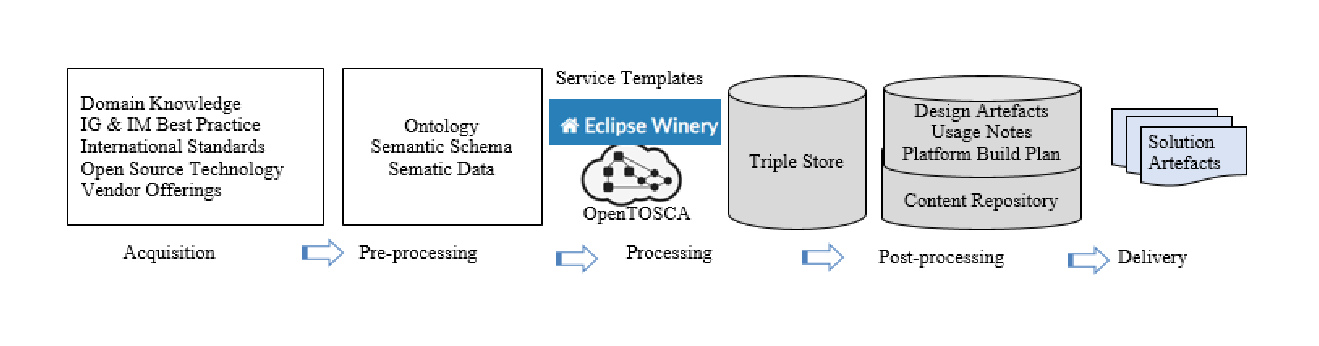
\includegraphics[width=\ScaleIfNeeded]{images/Bild1-2b.pdf}
    \caption{Process pipeline from knowledge acquisition to service implementation.}
  \label{fig:procpipe}
\end{figure*}
%\twocolumn
%\clearpage
\subsection{{Governance Domains}}
Governance at its core is about corporate and regulatory compliance. It is based on trust fueled by continuous IG practice, monitoring its effectiveness and control. This implies responsibilities and commitments realized through processes that ensure proper data access, implement guidelines and legal requirements. As such, corporate governance (CG) in an enterprise ensures that valuable information adhere with proper quality standards related to data authenticity, integrity and reliability in compliance with regulations. Thus enterprises are governed by a framework of principles, values, policies and processes intended to help organizational units to move towards shared corporate compliance goals. 
The principal design criteria of governance have a focus on enabling information quality strategies and to classify process capabilities against an Information Governance Maturity Model (Pierce, 2007). This means, at its core governance models cover three major responsibility domains: Corporate Governance (CG), Information Governance (IG) and IT Governance (ITG) outlined in Figure 2. Each domain addresses different governance areas using frameworks suitable for one or the other, emphasizing more the organizational or implementation aspects. 
The left-hand side of Figure 2 shows Information Governance and its relations to the categories of Information Management, Content Management, Records Management and Asset Management. These categories represent the context in which data is processed under the scrutiny of information governance lifecycles. The latter being workflows that perform activities to apply compliance policies and enforce rules on how to handle corporate data and information. Similarly, IT Governance, as shown on the right-hand side, relates to IT-Operations rules applied to infrastructure, processes. Thus, in the end governance means to enforce corporate compliance goals ensuring accountability and transparency such to minimize possible risks. 
The focus of the remainder of this paper is on information governance (IG) with occasional references to the other domains, where required.

%\vfill
\subsection{Problem Description}
From experience we learned that the success of information governance and regulatory compliance in companies depends on a common understanding conveyed through an unambiguous language. Such a language is an important pre-requisite to design, implementation and deployment of the required data governance services and their controls. In addition, an information governance strategy depends also on the type of data processed and the business context they belong to. For organizations this implies a responsibility to implement information governance practices that enforce proper data usage in their specific production environment throughout the entire information lifecycle. 
The problem though is that even after knowing ‘what is’ required, many companies face challenges with the architecture design of their individual IG solution because of the many technology and product options available on the market. 
These circumstances translate into a lengthy and formal process of announcing new information governance projects through a Request for Proposal (RFP) where in response, qualified contractors submit bids to undertake the project. Typically, the RFP document contains detailed information about the project, requirements, and evaluation criteria. 
The good news is that typical information governance solutions follow on an architecture blueprint that is composed of well-known software design patterns, available domain knowledge and experience. Luckily enough, software instances of IG building blocks are available in a variety of IG product offerings from open source and different vendors. Therefore, our conclusion is that by exploiting the available knowledge it is possible to generate the required information on components and design artefacts and allowing companies to compose IG solutions instead of custom developing new ones. Which is the goal of our approach outlined in Figure 1. This motivate the use of ontologies and knowledge graphs to store domain knowledge and to make it available through semantic search. The expected benefit is that on a global and open information market this knowledge facilitates the sharing of data and services. We think ontologies can expedite access and retrieval of IG service building blocks where the requirements defined in concept entities are matched by the capabilities of design entities. 
%
\begin{figure}[h]
  \centering
%    \includegraphics[clip, trim=1cm 7cm 0 0 , width=7.5cm]{images/iceis-fig02.png}
    \includegraphics[clip, trim=1cm 7cm 0 0 , width=7.5cm]{images/Fig2-CG.Domains.png}
    \caption{Corporate Governance Domains.}
  \label{fig:igdomains}
\end{figure}
\\ Figure 2: Corporate governance domains

\subsection{Usage Scenario}
Let us look at a real-world IG use case scenario to better explain our approach. Assume a company having the following business requisites: 
•	Business Data: Personal Identifiable Information (PII), customer contractual data and related contextual information; 
•	Businesses domiciled in: US, EU; 
•	Jurisdictions: US, EU; 
•	Regulations: US Privacy Act, EU GDPR; 
Regulatory compliance with these business requisites translates into the following functional and non-functional requirements:
•	R1: Contractual and legal obligations require to collect and classify person and business data as well as related information from pre-contract and contract activities (the context). 
•	 R2: Data is persisted reliably, after verifying its authenticity and integrity. 
•	R3: Data is stored for as long as required by business, legislations and regulations. 
•	R4: Access to stored data is controlled by security and privacy policies. 
•	R5: Data is deleted or barred from access upon lapse of a storage period prescribed by business or legal instruments. 
Figure 3 outlines the use case scenario in form of a semantic graph which we subdivided into three functional arias: Governance (top), Implementation (middle) and Platform (bottom). Note: Capitalized terms printed in bold represent key domain concepts. 
The upper part outlines the business requisites and reads like this: at corporate level a Company has a business presence in the Countries: EU and US. Their Jurisdictions are regulated by the US Privacy Act (GSA, 2022)and the EU GDPR Regulations (EU, 2018). Thus, this Company by law must instate an IG-Program consisting of a number of governance principles that address at the least: Security, Privacy, Integrity and Authenticity concerns in order to reach a maturity level Essential (L3 of L5).
%
\begin{figure*}[!hbtp]
  \centering
%   \includegraphics[width=\textwidth]{images/iceis-fig03.png}
   \includegraphics[width=\textwidth]{images/Fig3-IG.Scenario.png}
    \caption{Process pipeline from knowledge acquisition to service implementation.}
  \label{fig:igscenario}
\end{figure*}
%
 This means, each category consists of a number of obligations and implementation requirements to be satisfied. These are: 
•	R6: verify Data Authenticity, 
•	R7: ensure Data Integrity and 
•	R8: provide system and Service Reliability. 
From an implementation stand point these requirements translate into the following information governance guidelines:
 •	GL1: “…in order to reach a governance maturity Essential (level 3) an organization must implement a Metadata Definition Process that is an integral part of the implemented Records Management Practice”. See Figure 3.
 In addition, the US Privacy Act mandates that:
 •	GL2: “… Data integrity failures must be monitored, assessed, and mitigated …”.  
The center of Figure 3 lists the concept classes mentioned in the guidelines: Data, Metadata, and Records Management Practice. They all relate to processes that satisfy the associated requirements by means of inferred implementation and platform components. For example: Repository, RDBMS, Content Services as shown on the bottom of  Figure 3 
%
The line of thought at concept level follows this logic: The Metadata Definition Process is responsible for creating necessary governance metadata that describe how data is processed and stored based on applicable corporate and regulatory Policies. 
By following well known domain best practices, implementing such an IG-Program implies the presence of repositories where Data and related Metadata is securely stored. In this context, data is subject to different Lifecycles and controlled by a Records Management System. 
Records Classification processes classify the data in to categories and assign specific policies used to control classification, access, retention and disposition by means of appropriate Rules. 
Corporate repositories typically use Databases, Full Text Indexes and Storage Systems representing IT-Resources that today are best provisioned by Platform Services. 
 In a subsequent refinement step the IG concepts are then mapped on to solution component models and implementation classes where concept links are translated into class relationships. For example, following nodes at the bottom of Figure 3 one gets: 
Repository -> Content Repository-> Content Services -> Alfresco Content Services  •	Repository -> Metadata Repository -> Database Service -> Database ->PostgreSQL. 
With this approach, it is possible to identify the required components and design an IG solution following the architecture blueprint shown in Figure 4. From left to right, Figure 4 outlines how data is processed. Starting from the data sources where data is pre-processed and classified. Qualified data is then collected and loaded in an enterprise information systems (EIS) and put under control of information lifecycles. Governance lifecycle processes create required governance metadata before both data and metadata are persisted in an enterprise repository typically a Content Management (ECM) system. Post-processing, shown on the right side of Figure 4, is performed by Enterprise Records, Case Management, eDiscovery and Content Analytics components.  These services produce required governance information such to satisfy audit trails, statistics and reporting needs. 
At the high level Figure 3 represents the concept and  Figure 4  the implementation domain describing the mapping between concept, classes and components. The gist of what this use case is trying to convey is that with the given business requisites and based on the defined semantic model, it is possible to generate concept artefacts having the capabilities and characteristics for satisfying the implied functional, non-functional and operational requirements with the aid of a knowledge store. 
In summary we observe that a successful IG-Program implementation depends directly on an efficient enterprise information system where governance is achieved through adjustments of the information management practice with ongoing monitoring, assessment and reporting.